\subsection*{Problema 28}

\textbf{Enunciado:} 
Calcular la integral indefinida:
\begin{align*}
    I = \int x^3 (a + b x^3)^{1/4} \, dx
\end{align*}

\textbf{Solución:} 
Este es un caso de integración de diferenciales binomios de la forma:
\begin{align*}
    \int x^m (a + b x^n)^p \, dx
\end{align*}
donde $m = 3$, $n = 3$, y $p = 1/4$. 
Verificamos las condiciones de Chebyshev:
\begin{align*}
    \dfrac{m + 1}{n} &= \dfrac{3 + 1}{3} = \dfrac{4}{3} \quad (\text{no entero})
\end{align*}
Como $\dfrac{m + 1}{n}$ no es un número entero, probamos con la segunda condición:
\begin{align*}
    \dfrac{m + 1}{n} + p &= \dfrac{4}{3} + \dfrac{1}{4} = \dfrac{19}{12} \quad (\text{tampoco es entero})
\end{align*}
Por tanto, aplicamos un cambio de variable directo sobre el binomio interior para simplificar la potencia fraccionaria. Sea:
\begin{align*}
    u &= a + b x^3 \\
    u - a &= b x^3 \\
    x^3 &= \dfrac{u - a}{b}
\end{align*}

Diferenciando ambos lados:
\begin{align*}
    3 b x^2 \, dx &= du \\
    x^2 \, dx &= \dfrac{du}{3 b}
\end{align*}

Reorganizamos el integrando para hacer aparecer $x^2 \, dx$:
\begin{align*}
    I &= \int x \cdot (x^3) \cdot (a + b x^3)^{1/4} \, dx \\
    I &= \int (a + b x^3)^{1/4} \cdot x^3 \cdot (x^2 \, dx)
\end{align*}

Sustituimos las expresiones en términos de $u$:
\begin{align*}
    I &= \int u^{1/4} \left( \dfrac{u - a}{b} \right) \left( \dfrac{du}{3 b} \right) \\
    I &= \dfrac{1}{3 b^2} \int u^{1/4} (u - a) \, du \\
    I &= \dfrac{1}{3 b^2} \int (u^{5/4} - a u^{1/4}) \, du
\end{align*}

integramos cada término usando la regla de la potencia:
\begin{align*}
    I &= \dfrac{1}{3 b^2} \left[ \dfrac{u^{9/4}}{9/4} - a \dfrac{u^{5/4}}{5/4} \right] + C \\
    I &= \dfrac{1}{3 b^2} \left[ \dfrac{4}{9} u^{9/4} - \dfrac{4a}{5} u^{5/4} \right] + C
\end{align*}

Multiplicando por la constante exterior:
\begin{align*}
    I &= \dfrac{4}{27 b^2} u^{9/4} - \dfrac{4a}{15 b^2} u^{5/4} + C
\end{align*}

Finalmente, devolvemos la sustitución original $u = a + b x^3$:
\begin{align*}
    I &= \dfrac{4}{27 b^2} (a + bx^3)^{9/4} \\
      &\quad - \dfrac{4a}{15 b^2} (a + bx^3)^{5/4} + C
\end{align*}

\begin{figure}[H]
	\centering
	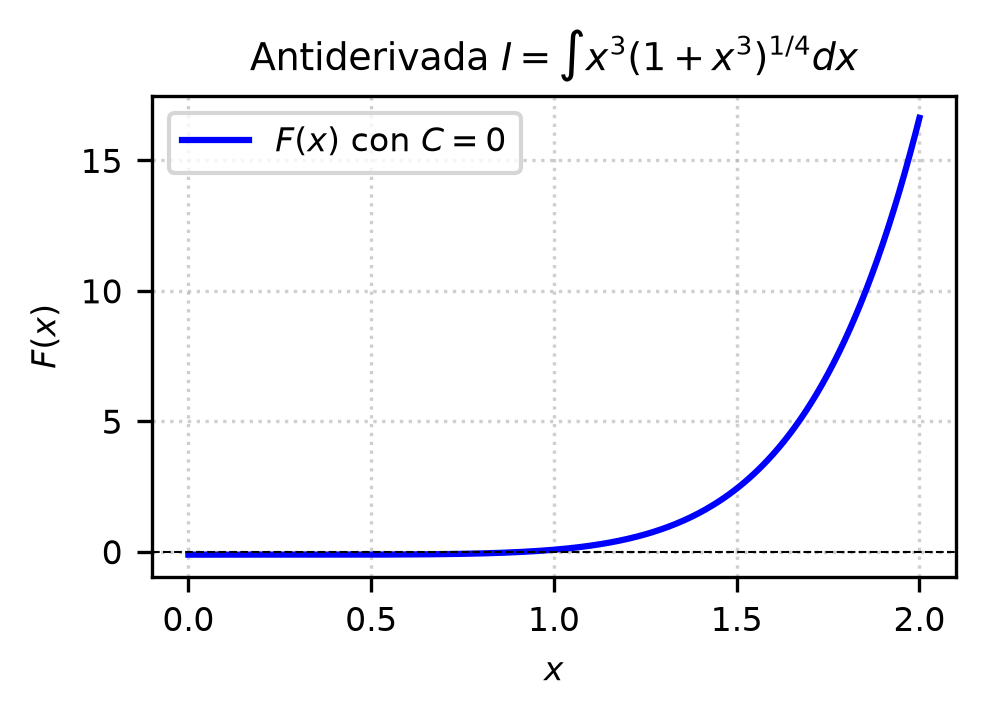
\includegraphics[width=\columnwidth]{semana_05/graficas/SEM05_P28_grafica.png}
	\caption{Representación gráfica de $f(x)$ y su antiderivada $F(x)$ evaluada para la constante de integración $C = 0$ (Problema 28).}
	\label{fig:problema28}
\end{figure}
